\documentclass{article}
\usepackage{amsmath}
\usepackage{breqn}
\usepackage{amssymb}

\usepackage{geometry}
\geometry{margin=1in}

\usepackage{hyperref}
\hypersetup{
    colorlinks=true,
    linkcolor=black,
    filecolor=magenta,      
    urlcolor=cyan,
    pdfpagemode=FullScreen,
}

\usepackage{graphicx}
\graphicspath{ {./images/} }


\begin{document}
\begin{titlepage}
    \begin{center}
        \vspace*{1cm}
            
        \Huge
        \textbf{Title}
            
        \vspace{0.5cm}
        \LARGE
        Subtitle
            
        \vspace{1.5cm}
            
        \textbf{Edgar Maddocks}
            
        \vfill
            
        \vspace{0.8cm}
                        
        \Large
        Bedford School\\
        03/05/2024\\
            
    \end{center}
\end{titlepage}

    \pagebreak

    \tableofcontents

    \section{Analysis}
    \subsection{Background}

    \subsection{Evidence of Analysis}

    \subsection{Current Systems}

    \subsection{Identification of end-user}

    \subsection{Modelling of the problem}

    \subsection{Set of objectives}

    \section{Research Log}
    \url{https://www.mastersofgames.com/rules/draughts-rules.htm}

    Rules of draughts

    \noindent \url{https://www.ibm.com/topics/neural-networks}

    A neural network is a machine learning model which aims to mimic the processes of the human brain.
    Each network contains inputs and outputs, as well as one or more layers of hidden nodes - which act as artificial neurons.
    In a fully connected network, each node is connected once to each node in the next layer - an example of how one node connects
    to the next layer can be seen in the image below.

    \begin{figure}[h]
        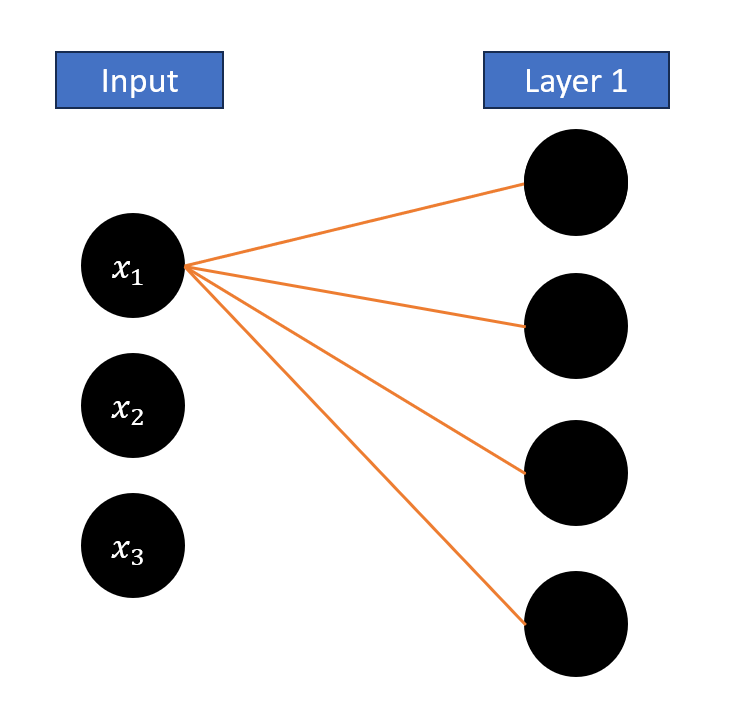
\includegraphics[scale=0.3]{ConnectedNode.png} 
        \centering
    \end{figure}

    Neural networks are a supervised learning model, meaning that they learn from labeled data (which has the objective correct answer in the data).
    They are sometimes referred to as artificial neural networks (ANNs) or simulated neural networks (SNNs).\\

    Neural networks can be modelled as a collection linear regression units.

    A single linear regression unit has the formula:

    \begin{displaymath}
        \hat{y} = \sum_{i=0}^{n} w_ix_i + b
    \end{displaymath}

    Where $\hat{y}$ is the predicted output, $n$ is the number of inputs, $x_i$ is the $i$th input, $w_i$ is the weight of $x_i$, and $b$ is a bias.
    If, for example, there were 3 inputs the full equation for $\hat{y}$ would be:
    
    \begin{displaymath}
        \hat{y} = w_1x_1 + w_2x_2 + w_3x_3 + b
    \end{displaymath}

    \noindent \url{https://courses.cs.washington.edu/courses/cse446/20wi/Lecture8/08_Regularization.pdf}

    This calculation can be vectorized to improve efficiency and would be notated:

    \begin{displaymath}
        \hat{y} = WX + b
    \end{displaymath}

    Where we let

    \begin{displaymath}
        W = \begin{bmatrix}
            w_1\\
            w_2\\
            \vdots\\
            w_n
        \end{bmatrix}\\
        \hspace{25px}
        X = \begin{bmatrix}
            x_1&
            x_2&
            \hdots&
            x_n
        \end{bmatrix}
    \end{displaymath}





    

    \noindent \url{https://www.turing.com/kb/mathematical-formulation-of-feed-forward-neural-network} Maths?

    \noindent \url{https://en.wikipedia.org/wiki/Automatic_differentiation} Automatic differentiation

    
    
\end{document}